% author:   sam tenka
% change:   2022-05-27
% create:   2022-05-11

%==============================================================================
%====  0.  DOCUMENT SETTINGS  ================================================
%==============================================================================

%~~~~~~~~~~~~~~~~~~~~~~~~~~~~~~~~~~~~~~~~~~~~~~~~~~~~~~~~~~~~~~~~~~~~~~~~~~~~~~
%~~~~~~~~~~~~~  0.0. About this Exposition  ~~~~~~~~~~~~~~~~~~~~~~~~~~~~~~~~~~~

%---------------------  0.0.0. page geometry  ---------------------------------
\documentclass[11pt, justified]{tufte-book}
\geometry{
  left           = 0.90in, % left margin
  textwidth      = 4.95in, % main text block
  marginparsep   = 0.15in, % gutter between main text block and margin notes
  marginparwidth = 2.30in, % width of margin notes
                 % 0.20in  % width from margin to edge
}

%---------------------  0.0.1. math packages  ---------------------------------
\newcommand\hmmax{0} % to allow for more fonts 
\newcommand\bmmax{0} % to allow for more fonts
\usepackage{amsmath, amssymb, amsthm, mathtools}
\usepackage{bm}
\usepackage{euler}

\usepackage{array}   % for \newcolumntype macro
\newcolumntype{L}{>{$}l<{$}} % math-mode version of "l" column type
\newcolumntype{C}{>{$}c<{$}} % math-mode version of "c" column type
\newcolumntype{R}{>{$}r<{$}} % math-mode version of "r" column type

%---------------------  0.0.2. graphics packages  -----------------------------
\usepackage{graphicx, xcolor}
\usepackage{float, capt-of}

%---------------------  0.0.3. packages for fancy text  -----------------------
\usepackage{enumitem}\setlist{nosep}
\usepackage{listings}
\usepackage{xstring}
\usepackage{fontawesome5}

%---------------------  0.043. colors  ----------------------------------------
\definecolor{mblu}{rgb}{0.05, 0.35, 0.70} \newcommand{\blu}{\color{mblu}}
\definecolor{mbre}{rgb}{0.30, 0.45, 0.60} \newcommand{\bre}{\color{mbre}}
\definecolor{mbro}{rgb}{0.60, 0.05, 0.05} \newcommand{\bro}{\color{mbro}}
\definecolor{mcya}{rgb}{0.10, 0.45, 0.45} \newcommand{\cya}{\color{mcya}}
\definecolor{mgre}{rgb}{0.55, 0.55, 0.50} \newcommand{\gre}{\color{mgre}}
\definecolor{mgrn}{rgb}{0.15, 0.65, 0.05} \newcommand{\grn}{\color{mgrn}}
\definecolor{mred}{rgb}{0.90, 0.05, 0.05} \newcommand{\red}{\color{mred}}

%~~~~~~~~~~~~~~~~~~~~~~~~~~~~~~~~~~~~~~~~~~~~~~~~~~~~~~~~~~~~~~~~~~~~~~~~~~~~~~
%~~~~~~~~~~~~~  0.1. Headers and References  ~~~~~~~~~~~~~~~~~~~~~~~~~~~~~~~~~~

%---------------------  0.1.0. intra-document references  ---------------------
\newcommand{\offour}[1]{
    {\tiny \raisebox{0.04cm}{\scalebox{0.9}{$\substack{
        \IfSubStr{#1}{0}{{\blacksquare}}{\square}   
        \IfSubStr{#1}{1}{{\blacksquare}}{\square} \\ 
        \IfSubStr{#1}{2}{{\blacksquare}}{\square}   
        \IfSubStr{#1}{3}{{\blacksquare}}{\square}   
    }$}}}%
}

\newcommand{\offourline}[1]{
    {\tiny \raisebox{0.04cm}{\scalebox{0.9}{$\substack{
        \IfSubStr{#1}{0}{{\blacksquare}}{\square}   
        \IfSubStr{#1}{1}{{\blacksquare}}{\square}
        \IfSubStr{#1}{2}{{\blacksquare}}{\square}   
        \IfSubStr{#1}{3}{{\blacksquare}}{\square}   
    }$}}}%
}
\newcommand{\notesam}[1]{{\blu \textsf{#1}}}
\newcommand{\attn}[1]{{\bro \textsf{#1}}}
\newcommand{\attnsam}[1]{{\red \textsf{#1}}}

\newcommand{\blarr}{\hspace{-0.15cm}${\bro \leftarrow}\,$}
\newcommand{\bcirc}{${\bro ^\circ}$}

\newcounter{footprintssofar}
\setcounter{footprintssofar}{90}
%\newcommand{\plainfootprint}{{\bro \rotatebox{\value{footprintssofar}}{\faIcon{shoe-prints}}}\setcounter{footprintssofar}{\value{footprintssofar}+30} }
\newcommand{\plainfootprint}{}
\newcommand{\footprint}{\marginnote{\plainfootprint} }

%---------------------  0.1.1. table of contents helpers  ---------------------
\newcommand{\phdot}{\phantom{.}}

%---------------------  0.1.2. section headers  -------------------------------
\newcommand{\samtitle} [1]{
  \par\noindent{\Huge \sf \blu #1}
  \vspace{0.4cm}
}

\newcommand{\samquote} [2]{
    \marginnote[-0.4cm]{\begin{flushright}
    \scriptsize
        \gre {\it #1} \\ --- #2
    \end{flushright}}
}

\newcommand{\samsection} [1]{
  \vspace{0.5cm}
  \par\noindent{\LARGE \sf \blu #1}
  \vspace{0.1cm}\par
}

\newcommand{\samsubsection}[1]{
  \vspace{0.3cm}
  \par\noindent{\Large \sf \bre #1}
  \vspace{0.1cm}\par
}

\newcommand{\samsubsubsection}[1]{
   \vspace{0.1cm}
   \par\noindent{\hspace{-2cm}\normalsize \sc \gre #1} ---
}

%---------------------  0.1.3. clear the bibliography's header  ---------------
\usepackage{etoolbox}
\patchcmd{\thebibliography}{\section*{\refname}}{}{}{}

%~~~~~~~~~~~~~~~~~~~~~~~~~~~~~~~~~~~~~~~~~~~~~~~~~~~~~~~~~~~~~~~~~~~~~~~~~~~~~~
%~~~~~~~~~~~~~  0.2. Math Symbols and Blocks  ~~~~~~~~~~~~~~~~~~~~~~~~~~~~~~~~~

%---------------------  0.2.0. general math operators  ------------------------
\newcommand{\scirc}{\mathrel{\mathsmaller{\mathsmaller{\mathsmaller{\circ}}}}}
\newcommand{\cmop}[2]{{(#1\!\to\!#2)}}

%---------------------  0.2.1. probability symbols  ---------------------------
\newcommand{\KL}{\text{KL}}
\newcommand{\EN}{\text{H}}
\newcommand{\note}[1]{{\blu \textsf{#1}}}

%---------------------  0.2.2. losses averaged in various ways  ---------------
\newcommand{\Ein}  {\text{trn}_{\sS}}
\newcommand{\Einb} {\text{trn}_{\check\sS}}
\newcommand{\Einc} {\text{trn}_{\sS\sqcup \check\sS}}
\newcommand{\Egap} {\text{gap}_{\sS}}
\newcommand{\Eout} {\text{tst}}

%---------------------  0.2.3. double-struck and caligraphic upper letters  ---
\newcommand{\Aa}{\mathbb{A}}\newcommand{\aA}{\mathcal{A}}
\newcommand{\Bb}{\mathbb{B}}\newcommand{\bB}{\mathcal{B}}
\newcommand{\Cc}{\mathbb{C}}\newcommand{\cC}{\mathcal{C}}
\newcommand{\Dd}{\mathbb{D}}\newcommand{\dD}{\mathcal{D}}
\newcommand{\Ee}{\mathbb{E}}\newcommand{\eE}{\mathcal{E}}
\newcommand{\Ff}{\mathbb{F}}\newcommand{\fF}{\mathcal{F}}
\newcommand{\Gg}{\mathbb{G}}\newcommand{\gG}{\mathcal{G}}
\newcommand{\Hh}{\mathbb{H}}\newcommand{\hH}{\mathcal{H}}
\newcommand{\Ii}{\mathbb{I}}\newcommand{\iI}{\mathcal{I}}
\newcommand{\Jj}{\mathbb{J}}\newcommand{\jJ}{\mathcal{J}}
\newcommand{\Kk}{\mathbb{K}}\newcommand{\kK}{\mathcal{K}}
\newcommand{\Ll}{\mathbb{L}}\newcommand{\lL}{\mathcal{L}}
\newcommand{\Mm}{\mathbb{M}}\newcommand{\mM}{\mathcal{M}}
\newcommand{\Nn}{\mathbb{N}}\newcommand{\nN}{\mathcal{N}}
\newcommand{\Oo}{\mathbb{O}}\newcommand{\oO}{\mathcal{O}}
\newcommand{\Pp}{\mathbb{P}}\newcommand{\pP}{\mathcal{P}}
\newcommand{\Qq}{\mathbb{Q}}\newcommand{\qQ}{\mathcal{Q}}
\newcommand{\Rr}{\mathbb{R}}\newcommand{\rR}{\mathcal{R}}
\newcommand{\Ss}{\mathbb{S}}\newcommand{\sS}{\mathcal{S}}
\newcommand{\Tt}{\mathbb{T}}\newcommand{\tT}{\mathcal{T}}
\newcommand{\Uu}{\mathbb{U}}\newcommand{\uU}{\mathcal{U}}
\newcommand{\Vv}{\mathbb{V}}\newcommand{\vV}{\mathcal{V}}
\newcommand{\Ww}{\mathbb{W}}\newcommand{\wW}{\mathcal{W}}
\newcommand{\Xx}{\mathbb{X}}\newcommand{\xX}{\mathcal{X}}
\newcommand{\Yy}{\mathbb{Y}}\newcommand{\yY}{\mathcal{Y}}
\newcommand{\Zz}{\mathbb{Z}}\newcommand{\zZ}{\mathcal{Z}}

%---------------------  0.2.4. sans serif and frak lower letters  -------------
\newcommand{\sfa}{\mathsf{a}}\newcommand{\fra}{\mathcal{a}}
\newcommand{\sfb}{\mathsf{b}}\newcommand{\frb}{\mathcal{b}}
\newcommand{\sfc}{\mathsf{c}}\newcommand{\frc}{\mathcal{c}}
\newcommand{\sfd}{\mathsf{d}}\newcommand{\frd}{\mathcal{d}}
\newcommand{\sfe}{\mathsf{e}}\newcommand{\fre}{\mathcal{e}}
\newcommand{\sff}{\mathsf{f}}\newcommand{\frf}{\mathcal{f}}
\newcommand{\sfg}{\mathsf{g}}\newcommand{\frg}{\mathcal{g}}
\newcommand{\sfh}{\mathsf{h}}\newcommand{\frh}{\mathcal{h}}
\newcommand{\sfi}{\mathsf{i}}\newcommand{\fri}{\mathcal{i}}
\newcommand{\sfj}{\mathsf{j}}\newcommand{\frj}{\mathcal{j}}
\newcommand{\sfk}{\mathsf{k}}\newcommand{\frk}{\mathcal{k}}
\newcommand{\sfl}{\mathsf{l}}\newcommand{\frl}{\mathcal{l}}
\newcommand{\sfm}{\mathsf{m}}\newcommand{\frm}{\mathcal{m}}
\newcommand{\sfn}{\mathsf{n}}\newcommand{\frn}{\mathcal{n}}
\newcommand{\sfo}{\mathsf{o}}\newcommand{\fro}{\mathcal{o}}
\newcommand{\sfp}{\mathsf{p}}\newcommand{\frp}{\mathcal{p}}
\newcommand{\sfq}{\mathsf{q}}\newcommand{\frq}{\mathcal{q}}
\newcommand{\sfr}{\mathsf{r}}\newcommand{\frr}{\mathcal{r}}
\newcommand{\sfs}{\mathsf{s}}\newcommand{\frs}{\mathcal{s}}
\newcommand{\sft}{\mathsf{t}}\newcommand{\frt}{\mathcal{t}}
\newcommand{\sfu}{\mathsf{u}}\newcommand{\fru}{\mathcal{u}}
\newcommand{\sfv}{\mathsf{v}}\newcommand{\frv}{\mathcal{v}}
\newcommand{\sfw}{\mathsf{w}}\newcommand{\frw}{\mathcal{w}}
\newcommand{\sfx}{\mathsf{x}}\newcommand{\frx}{\mathcal{x}}
\newcommand{\sfy}{\mathsf{y}}\newcommand{\fry}{\mathcal{y}}
\newcommand{\sfz}{\mathsf{z}}\newcommand{\frz}{\mathcal{z}}

%---------------------  0.2.5. math environments  -----------------------------
\newtheorem*{qst}{Question}
\newtheorem*{thm}{Theorem}
\newtheorem*{lem}{Lemma}
% ...
\theoremstyle{definition}
\newtheorem*{dfn}{Definition}

%==============================================================================
%=====  1.  PROLOGUE  =========================================================
%==============================================================================

\begin{document}
%\samtitle{recitation 01 (optional 6.86x notes)}
\samtitle{optional 6.86x notes}

      %\marginnote{%
      %  %These notes overlap with what we'll cover in recitation.  But
      %  Recitation has more coding and less theory than these notes.
      %  %We'll
      %  %skip whole passages of these notes during recitation.
      %  %
      %  Footprints --- \plainfootprint --- roughly indicate our pacing: we'll
      %  linger on the points near each footprint for three to seven
      %  minutes.
      %  %
      %  %A recitation might have eighteen footprints.
      %}

      \attn{You do not need to read these notes at all} to get an A
      in this course; conversely, \attn{you may not cite these notes} when
      solving homework or exams.
       
  \samsection{A. prologue}
    \samquote{
      I shall create! If not a note, a hole.  If not an overture, a
      desecration.
    }{gwendolyn brooks}
    %\samquote{
    %  One beginning and one ending for a book was a thing I did not agree
    %  with.  A good book may have three openings entirely dissimilar ...
    %}{flann o'brien}

    \samsubsection{bird's eye view}
 
      \samsubsubsection{kinds of learning}
        How do we communicate patterns of desired behavior?  We can teach:\footprint
        \begin{description}
          \item[\textbf{by instruction}:  ]  ``to tell whether a mushroom is poisonous, first look at its gills...'' 
          \item[\textbf{by example}:      ]  ``here are six poisonous fungi; here, six safe ones.  see a pattern?''
          \item[\textbf{by reinforcement}:]  ``eat foraged mushrooms for a month; learn from getting sick.''
        \end{description}
        %
        \marginnote{%
          \attn{Exercise:} What's a thing you know now but not last month?
          What kinds of signal taught you?
        }
        Machine learning is the art of programming computers to learn from such
        sources.  We'll focus on the most important case: learning from
        examples.\bcirc\marginnote{%
          \blarr In Unit 5 of 6.86x, we'll see that learning by example is key to
          the other modes of learning.
        }

      \samsubsubsection{from examples to predictions}
        For us, a pattern of desired behavior is a function that for each given
        situation/prompt returns a favorable action/answer.\footprint
        %
        Our goal is to write a program that, from a list of $N$ examples of
        prompts and matching answers, determines an underlying pattern.  We
        consider our program a success if this pattern accurately predicts
        answers corresponding to new, unseen prompts.
        %
        We often define our program as a search, over some set $\hH$ of
        candidate patterns, to minimize some notion of ``discrepancy from the
        example data''.\footprint

        \begin{figure}[h]
          \vspace{-0.5cm}
          \par\noindent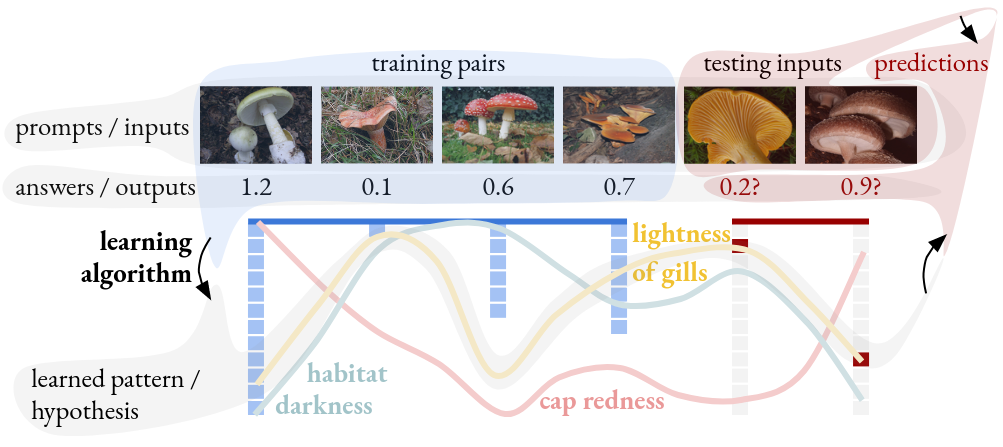
\includegraphics[width=\textwidth]{figures/supervised}\\
          \caption{%
            A program that learns to predict mushrooms' poison levels:
            %
            first takes a list of labeled mushrooms as input (blue blob);
            searches
            through candidate patterns (here, the wiggly curves labeled
            \texttt{lightness of gills}, \texttt{habitat darkness}, and
            \texttt{cap redness}); and returns the pattern that best fits the
            examples.
            %
            Evaluating this pattern on new mushrooms, we predict their poison
            levels (red blob). 
            %
            \par The three bold black arrows show the flow of data from
            training examples to a learned pattern; and from that pattern
            together with testing prompts to predictions.  
            %
            Part of specifying the learning program is specifying the set of candidate patterns to consider.
          }
          \vspace{-0.5cm}
        \end{figure}

        To save ink, say that $\xX$ is the set of possible prompts; $\yY$, of
        possible answers.\bcirc\marginnote{%
          \blarr If we like, we can now summarize the data flow in symbols.  A
          pattern is a function of type $\xX\to\yY$.  And we can model the
          examples from which our program learns as a list of type $(\xX\times
          \yY)^N$.  Then a program that learns from examples has type:
          $$
            \lL : (\xX\times \yY)^N \to (\xX\to \yY)
          $$
          Once we allow uncertainty by letting patterns map to \emph{probability
          distributions} over answers, the type will change to:
          $$
            \lL : (\xX\times \yY)^N \to (\xX\to \text{DistributionsOn}(\yY))
          $$
        }
        In the mushrooms example, $\xX$ contains all
        conceivable mushrooms and $\yY$ contains all conceivable poison
        levels (perhaps all the non-negative real numbers).

      \samsubsubsection{supervised learning}
        We'll soon allow uncertainty by letting patterns map to \emph{probability
        distributions} over answers.
        %
        Even if the prompt is always the same --- say, ``produce a beautiful
        melody'', we may seek to understand the complicated distribution over
        answers.  We might regard our program a success if it can
        generate a variety of good answers.
        %
        So-called \textbf{unsupervised learning} focuses in that way on output
        structure.  By contrast, \textbf{supervised learning} (our subject in
        Unit 1), focuses on the input-output relation; it's interesting when
        the space of prompts is large.\footprint
        %

    \newpage
    \samsubsection{a tiny example: handwritten digit classification}
      \samquote{
        The learning process is something you can incite, literally incite, like a riot.
      }{audre lorde}

      \samsubsubsection{meeting the data}
        $\xX = \{\text{grayscale~}28\!\times\!28\text{-pixel images}\}$;
        $\yY=\{{\cya{1}},{\red{9}}\}$.  Each datum $(x,y)$ arises as follows:
        we randomly choose a digit $y\in \yY$, ask a human to write that digit
        in pen, and then photograph their writing to produce $x\in\xX$.\footprint
        %
        \vspace{-0.25cm}
        \begin{figure}
            \centering
          \begin{tabular}{c}
\includegraphics[width=0.75cm]{example-mnist/mnist-trn-00}\\$\red{9}$\\
\includegraphics[width=0.75cm]{example-mnist/mnist-trn-10}\\$\cya{1}$\end{tabular}%
          \begin{tabular}{c}
\includegraphics[width=0.75cm]{example-mnist/mnist-trn-01}\\$\cya{1}$\\
\includegraphics[width=0.75cm]{example-mnist/mnist-trn-11}\\$\red{9}$\end{tabular}%
          \begin{tabular}{c}
\includegraphics[width=0.75cm]{example-mnist/mnist-trn-02}\\$\red{9}$\\
\includegraphics[width=0.75cm]{example-mnist/mnist-trn-12}\\$\cya{1}$\end{tabular}%
          \begin{tabular}{c}
\includegraphics[width=0.75cm]{example-mnist/mnist-trn-03}\\$\red{9}$\\
\includegraphics[width=0.75cm]{example-mnist/mnist-trn-13}\\$\cya{1}$\end{tabular}%
          \begin{tabular}{c}
\includegraphics[width=0.75cm]{example-mnist/mnist-trn-04}\\$\cya{1}$\\
\includegraphics[width=0.75cm]{example-mnist/mnist-trn-14}\\$\red{9}$\end{tabular}%
          \begin{tabular}{c}
\includegraphics[width=0.75cm]{example-mnist/mnist-trn-05}\\$\red{9}$\\
\includegraphics[width=0.75cm]{example-mnist/mnist-trn-15}\\$\red{9}$\end{tabular}%
          \begin{tabular}{c}
\includegraphics[width=0.75cm]{example-mnist/mnist-trn-06}\\$\red{9}$\\
\includegraphics[width=0.75cm]{example-mnist/mnist-trn-16}\\$\red{9}$\end{tabular}%
          \begin{tabular}{c}
\includegraphics[width=0.75cm]{example-mnist/mnist-trn-07}\\$\red{9}$\\
\includegraphics[width=0.75cm]{example-mnist/mnist-trn-17}\\$\cya{1}$\end{tabular}%
          \begin{tabular}{c}
\includegraphics[width=0.75cm]{example-mnist/mnist-trn-08}\\$\cya{1}$\\
\includegraphics[width=0.75cm]{example-mnist/mnist-trn-18}\\$\red{9}$\end{tabular}%
          \begin{tabular}{c}
\includegraphics[width=0.75cm]{example-mnist/mnist-trn-09}\\$\red{9}$\\
\includegraphics[width=0.75cm]{example-mnist/mnist-trn-19}\\$\cya{1}$\end{tabular}%
          \caption{
            Twenty example pairs.  Each photo $x$ is a $28\times 28$ grid of
            numbers representing pixel intensities.  The light gray background
            has intensity $0.0$; the blackest pixels, intensity $1.0$.  Below
            each photo $x$ we display the corresponding label $y$:
            either $y= {\cya{1}}$ or
            $y={\red{9}}$.
            %
            We'll adhere to this color code throughout this tiny example.
          }
        \end{figure}

        \begin{marginfigure}
          \vspace{-3.5cm}
          
\includegraphics[width=0.47\textwidth]{example-mnist/mnist-trn-00}%\\$\red{9}$
            \hspace{0.03\textwidth}
          
\includegraphics[width=0.47\textwidth]{example-mnist/mnist-trn-01}%\\$\cya{1}$
        \end{marginfigure}
        When we zoom in, we can see each photo's $28\times 28$ grid of pixels.
        On the computer, this data is stored as a $28\times 28$ grid of numbers:
        $0.0$ for bright through $1.0$ for dark.
        Our convention will be to name these $28\times28$ grid locations by the
        number of their row (counting starting from the top) and then of their
        column (counting starting from the left).  So location $(0,0)$ is the
        upper left corner pixel; location $(27,0)$ is the lower left corner
        pixel.
        \par\noindent
        \attn{Exercise:} {Where is location $(0,27)$?  %$(14,8)$?
        In which direction is $(14,14)$ off-center?}
        \par\noindent
        \attn{Exercise:} {What pixel intensities do these two photos have at these  %three
        two locations?}

        \footprint
        As part of getting to know the data, it's worth taking a moment to
        think about how we would go about hand-coding a digit classifier.  The
        challenge is to complete the pseudocode
        %
        ``\texttt{if (?)\ then predict y=9 else predict y=1}''.
        %
        Well, ${\red{9}}$s tend to have more ink than than ${\cya{1}}$s ---
        should \texttt{(?)}\ threshold by the photo's darkness?
        %
        Or: ${\cya{1}}$s and ${\red{9}}$s tend to have different heights ---
        should \texttt{(?)}\ threshold by the photo's dark part's height?

        \begin{marginfigure}
          \centering
          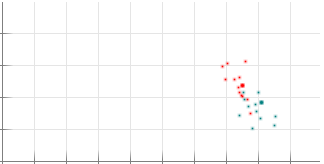
\includegraphics[width=0.99\textwidth]{example-mnist/train-plain}
          \caption{
            Our size-$N=25$ set of training examples, viewed in the
            darkness-height plane.  The vertical \emph{darkness} axis ranges
            $[0.0,0.25]$; the horizontal \emph{height} axis ranges $[0.0,0.5]$.
            The origin is at the lower left.  Each {\cya{cyan}} dot represents a
            $y={\cya{1}}$ example; each {\red{red}} dot, a $y={\red{9}}$ one.
            %
            The big ${\red{9}}$ above has darkness and height $(0.118, 0.375)$;\
            the big ${\cya{1}}$, $(0.092, 0.404)$.  See where they are in this
            plot?
          }
        \end{marginfigure}

        To make this precise, let's define a photo's \emph{darkness} as its
        average pixel darkness; its \emph{height} as the standard deviation of
        the row index of its dark pixels.  For convenience let's normalize
        both height and darkness to have max possible value $1.0$.  Such
        functions from inputs in $\xX$ to numbers are called
        \textbf{features}.\footprint

        \begin{lstlisting}[language=Python, basicstyle=\footnotesize\ttfamily]
          SIDE = 28
          def darkness(x):
            return np.mean(np.mean(x, axis=0), axis=0)
          def height(x):
            return np.std([row for col in range(SIDE)
                               for row in range(SIDE)
                               if 0.5 < x[row][col]  ])/(SIDE/2.0) 
        \end{lstlisting}

        So we can threshold by darkness or by height.  But this isn't very
        satisfying, since sometimes there are especially dark ${\cya{1}}$s or
        tall ${\red{9}}$s. 
        %
        We thus arrive at the idea of using \emph{both} features: ${\red{9}}$s
        are darker than ${\cya{1}}$s \emph{even relative to their
        height}.  So we might write something like
        \texttt{2*darkness(x)-height(x)>0} for\bcirc\marginnote{%
          \blarr That factor of $2$ comes from our observation that darkness
          tends to be bigger than height.  We'll soon see that this eyeballed
          slope doesn't work well.  It's better to tune by machine.
        } our condition.

        \begin{lstlisting}[language=Python, basicstyle=\footnotesize\ttfamily]
          def hand_coded_predict(x):
            return 9 if 2*darkness(x)-height(x)>0 else 1
        \end{lstlisting}

        \noindent
        \attn{Exercise:} {Beyond height and darkness, what features do you think
        might help us to separate digits $1$ from $9$?}\footprint

    \newpage
      \samsubsubsection{candidate patterns}
        We can generalize the hand-coded hypothesis from the previous passage
        to other coefficients besides $1\cdot \text{height}(x) -
        2\cdot\text{darkness}(x)$.  We let our set $\hH$ of candidate patterns
        contain all ``linear hypotheses'' $f_{a,b}$ defined by:\footprint
        $$
          f_{a,b}(x) = {\red{9}} \text{~~if~~} a\cdot\text{darkness}(x) + b\cdot\text{height}(x) > 0 \text{~~else~~} {\cya{1}}
        $$ 
        Each $f_{a,b}$ makes predictions of $y$s given $x$s.  As we change $a$
        and $b$, we get different predictors, some more accurate than others.

        \begin{lstlisting}[language=Python, basicstyle=\footnotesize\ttfamily]
          def predict(x,a,b):
            return 9 if a*darkness(x) + b*height(x) > 0 else 1
        \end{lstlisting}

        \noindent
        \attn{Exercise:} {Fig \ref{fig:train-test-digits}: match up $\offourline{0}$'s $3$ lines with
        $\offourline{1}$'s $3$ boxed points.}\footprint

      \samsubsubsection{optimization}
        Let's write a program $\lL$ that given a list of \emph{training
        examples} produces a hypothesis in $h \in \hH$ that helps us predict
        the labels $y$ of yet-unseen photos $x$ (\emph{testing examples}).
        Insofar as training data is representative of testing data, it's
        sensible to return a $h\in \hH$ that correctly classifies maximally
        many training examples.\footprint
        %
        To do this, let's make $\lL$ loop over all integer pairs $(a,b)$ in
        $[-99,+99]$:  %to minimize the number of misclassified training examples. 
        \begin{lstlisting}[language=Python, basicstyle=\footnotesize\ttfamily]
          def accuracy_on(examples,a,b):
            return sum(1.0 for x,y in examples if predict(x,a,b)==y)/len(examples)

          def best_hypothesis():
            return max((accuracy_on(training_data, a, b), (a,b))
                       for a in range(-99,100) 
                       for b in range(-99,100))
        \end{lstlisting}

        \begin{figure}[h]
            \centering
            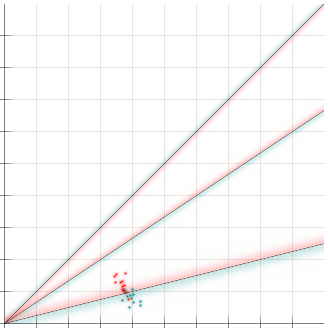
\includegraphics[width=0.23\textwidth]{example-mnist/new-train.png}%
            \hspace{0.01\textwidth}%
            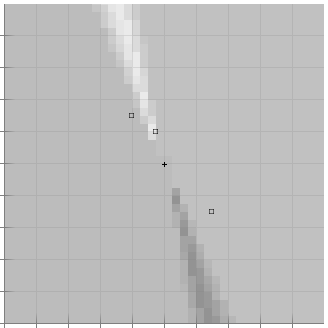
\includegraphics[width=0.23\textwidth]{example-mnist/new-train-scat.png}%
            \hspace{0.02\textwidth}%
            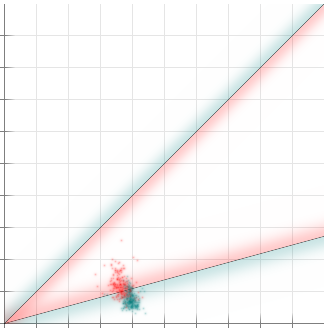
\includegraphics[width=0.23\textwidth]{example-mnist/new-test.png}%
            \hspace{0.01\textwidth}%
            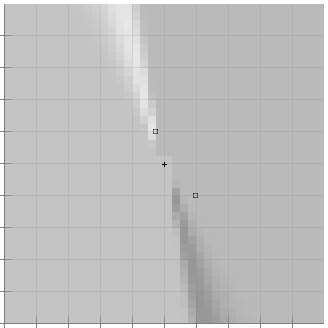
\includegraphics[width=0.23\textwidth]{example-mnist/new-test-scat.png}
            %
            \caption{
              \textbf{Training
              ($\protect\offourline{01}$) and testing
              ($\protect\offourline{23}$).}
              %
              $3$ hypotheses classify training data in the darkness-height
              plane ($\protect\offourline{0}$); glowing colors distinguish a
              hypothesis' $\cya{1}$ and $\red{9}$ sides.
              %
              Each point in the $(a,b)$ plane ($\protect\offourline{1}$)
              represents a hypothesis; darker regions misclassify a greater
              fraction of training data.
              %
              Panes $\protect\offourline{23}$ show the same for
              \emph{testing} data.
              %
              $\protect\offourline{02}$'s axes range $[0, 1.0]$.
              $\protect\offourline{13}$'s axes range $[-99,+99]$. 
            }
            \label{fig:train-test-digits}
        \end{figure}


        When we feed $N=25$ training examples to $\lL$, it produces
        $(a,b)=(80,-20)$ as a minimizer of \textbf{training error}, i.e.,
        of the fraction of training examples misclassified.  It misclassifies
        only $12\%$ of training examples.\footprint Yet the same
        hypothesis misclassified a greater fraction --- $18\%$ --- of fresh,
        yet-unseen testing examples.
        %
        That latter number --- called the \textbf{testing error} --- represents
        our program's accuracy ``in the wild'';
        it's the number we most care about.  The difference between training
        and testing error is the difference between our score on a practice
        exam or homework, where we're allowed to review mistakes we made and
        do a second try, versus our score on an exam, where we don't know the
        questions beforehand and aren't allowed to change our answers once we
        get our grades back.

        \noindent
        \attn{Exercise:} {visualize $f_{a,b}$'s error on $N=1$ example as a 
        function of $(a,b)$.}\footprint

      \samsubsubsection{error analysis}
        Intuitively, our testing error of $18\%$ comes from three sources:
        \textbf{(a)} the failure of our training set to be representative of our testing set; 
        \textbf{(b)} the failure of our program to exactly minimize training error over $\hH$;
        \textbf{(c)} and the failure of our hypothesis set $\hH$ to contain ``the true'' pattern. 

        These are respectively errors of
        \textbf{generalization},
        \textbf{optimization},
        \textbf{approximation}.

        Here, we got optimization error $\approx 0\%$ (albeit by
        \emph{unscalable brute-force}).  Because optimization error is zero in
        our case, the approximation error and training error are the same:
        $\approx12\%$.  The approximation error is so high because our straight
        lines are \emph{too simple}: height and darkness lose useful
        information, and the ``true'' boundary between training digits looks
        curved.\footprint
        %
        Finally, our testing error $\approx 18\%$ exceeds our training error.
        We thus suffer a generalization error of $\approx 6\%$: we \emph{didn't
        perfectly extrapolate} from training to testing situations.
        %
        In 6.86x we'll address all three italicized issues.

        \noindent
        \attn{Exercise:} {why is generalization error usually positive?}\footprint

    %\newpage
    \samsubsection{supervised learning framework}
      \samquote{
        Everybody gets so much information all day long that they lose their
        common sense.
      }{gertrude stein}

      \samsubsubsection{formalism}
        Draw training examples $\sS : (\xX\times \yY)^N$ %a list of examples
        from nature's distribution $\dD$ on $\xX\times \yY$.  A pattern
        $f:\xX\to \yY$ has \textbf{training error}
        $
           \Ein(f) = \Pp_{(x,y)\sim \red{\sS}}[f(x)\neq y] 
        $, an average over examples; and \textbf{testing error}
        $
           \Eout(f) = \Pp_{(x,y)\sim \red{\dD}}[f(x)\neq y] 
        $, an average over nature.  A \emph{learning program} is a function 
        $
            \lL : (\xX\times \yY)^N \to (\xX\to \yY)
        $; we want to design $\lL$ so that it maps typical $\sS$s to $f$s with
        low $\Eout(f)$.\marginnote{%
          %  TODO: mention extereme class-imbalance and bayesian *decision* theory 
        }

      \samsubsubsection{learning error}
        As in the previous subsection's tiny example,  
        we often define
        $\lL$ to roughly
        minimize $\Ein$ over a
        set $\hH \subseteq (\xX\to \yY)$ of candidate patterns.  Then $\Eout$
        decomposes
        into the failures
        of
        $\Ein$ to estimate $\Eout$ (generalization),
        of
        $\lL$ to minimize $\Ein$ (optimization), and 
        of
        $\hH$ to contain
        nature's
        truth (approximation): 
        \newcommand{\minf}[1]{{\inf}_{\hH}}
        \begin{align*}
            \Eout(\lL(\sS)) 
            =~&\Eout(\lL(\sS))      &-\,\,\,&      \Ein(\lL(\sS)) &~\}~& \text{\textbf{generalization} error} \\
            +~&\Ein(\lL(\sS))       &-\,\,\,& \minf{\hH}(\Ein(f)) &~\}~& \text{\textbf{optimization} error} \\
            +~&\minf{\hH}(\Ein(f))  &       &                     &~\}~& \text{\textbf{approximation} error}  
        \end{align*}
        These terms are in tension.  For example, as $\hH$ grows, the
        approx.\ error may decrease while the gen.\ error may
        increase --- this is the ``\textbf{bias-variance} tradeoff''.

        %\marginnote{%
        %  \parbox{\textwidth}{
        %  \begin{lstlisting}[language=Python, basicstyle=\footnotesize\ttfamily]
        %    def width(x):
        %      return np.std([row for col in range(SIDE)
        %                         for row in range(SIDE)
        %                         if 0.5 < x[row][col]  ])/(SIDE/2.0) 
        %    def holiness(x):
        %      return np.mean([1 if (np.max(x[:row,:col]) > x[row,col] and 
        %                            np.max(x[:row,col:]) > x[row,col] and 
        %                            np.max(x[row:,:col]) > x[row,col] and 
        %                            np.max(x[row:,col:]) > x[row,col]    ) else 0
        %                        for col in range(1,SIDE-1)
        %                        for row in range(1,SIDE-1)                       ])
        %    def topheaviness(x):
        %      return (np.mean(x[:int(SIDE/2)])-np.mean(x[int(SIDE/2):]) + 1.0)/2 
        %    #def overlap_one(x):
        %    #  return np.sum()
        %    #def overlap_nine(x):
        %  \end{lstlisting}
        %  We normalized all features so that they output values in $[0.0,1.0]$. 
        %}
        %}



      \samsubsubsection{workflow}
      %\samsubsubsection{workflow: framing}
        We first \emph{frame}: what data will help us solve what problem?  To
        do this, we \emph{factor} our complex prediction problem into simple
        classification or regression problems; randomly \emph{split} the
        resulting example pairs into training, dev(elopment), and testing sets;
        and \emph{visualize} the training data to weigh our intuitions. 

      %\samsubsubsection{workflow: modeling}
        Next, we \emph{model}: we present the data to the computer so that
        true patterns are more easily found.
        %
        Here we inject our \emph{domain knowledge} --- our human experience and
        intuition about which factors are likely to help with prediction.
        %
        Modeling includes \emph{featurizing} our inputs and choosing
        appropriate \emph{priors} and \emph{symmetries}.

      %\samsubsubsection{workflow: training}
        During \emph{training}, the computer searches among candidate patterns
        for one that explains the examples relatively well.
        We used brute force above; we'll soon learn faster algorithms
        such as \emph{gradient descent} on the training set for parameter
        selection and \emph{random grid search} on the dev set for
        hyperparameter selection.

      %\samsubsubsection{workflow: harvesting}
        Finally, we may \emph{harvest}: we derive insights from the pattern
        itself\bcirc\marginnote{%
            \blarr which factors ended up being most important? 
        }
        and we predict outputs for to fresh inputs.
        %
        Qualifying both applications is the pattern's quality.  To assess this,
        we measure its accuracy on our held-out testing data.


\end{document}

